\section{Introduction}

\subsection{Chapter outline}

In this chapter I aim to characterise human microfilaria (mf) prevalence of lymphatic filariasis (LF) as a function of mosquito prevalence, describing a method of disease surveillance using different vector sampling and testing methods. I characterise uncertainty around my calculations and investigate the sample sizes required for xenomonitoring-derived estimates to be useful for public health decision-making. I also simulate the described sampling and human prevalence estimation process in an elimination setting (human mf prevalence of 1\%) to demonstrate feasibility and compare individual and pool-based sampling.

\subsection{Background}

With sixteen countries and territories having achieved validation of elimination of LF as a public health problem (EPHP), and seven more recently under post-MDA surveillance \cite{WHO2019_FactSheet}, there is increasing discussion on what should be done post-validation. As achieving EPHP is not necessarily expected to guarantee true elimination of transmission \cite{Rao2019}, and with the largely unknown risk of resurgence \cite{Xu2019,NTDMC2019}, there is a need for well formulated guidelines on what programs should be aiming to do after validation of EPHP. Currently the World Health Organization (WHO) requires a nation to pass three transmission assessment surveys (TAS1--3) and have some ongoing surveillance to achieve validation, but there is no guidance on what this ongoing surveillance should entail \cite{WHO2017_Validation}. This results in a real risk that some programs will stop effectively monitoring disease levels after achieving validation, potentially leading to undetected resurgence.

A number of countries have implemented their own post-validation strategies, including combinations of passive surveillance, active case tracing, focused testing of at-risk populations and vector surveys \cite{Rao2019,Dorkenoo2018,Irish2018,Pi2018}. Human diagnostics used are either antigen tests (immunochromatographic test, ICT, or filarial test strip, FTS) or microscopic examinations of night blood smears, although poor specificity in the antigen tests means some programs follow up any positives with night blood smears \cite{Rahman2019}. Entomological surveillance is currently described by the WHO as optional \cite{WHO2017_Validation}, but is being used as a tool to detect presence of infection in a number of post-validation settings including Ghana, Togo and Bangladesh \cite{Dorkenoo2018,Irish2018,Pi2018}. 

The main methods of testing vectors for disease are dissection \cite{Pi2018}, for identification of \textit{W. bancrofti} larval stages under a microscope, or real-time polymerase chain reaction (PCR) to identify presence of parasite DNA in mosquito carcasses, termed molecular xenomonitoring (MX) \cite{Dorkenoo2018,Irish2018}. Dissection is labour intensive and a positive result requires a viable infection in the mosquito, whereas with PCR it is possible to detect presence of \textit{W. bancrofti} DNA if a vector has simply taken a blood meal from an infected human \cite{Zaky2018}. PCR methods often involve grouping the mosquitoes into pools of 10 or more (known as pooling) to increase the accuracy of PCR outputs and save on costs. Other testing methods are also in development, including PCR testing of mosquito excreta that can detect whether a mosquito has taken an mf positive blood meal \cite{Pilotte2016}. 

Xenomonitoring is a non-invasive alternative to human surveys, and is potentially capable of indirectly measuring parasite burden within endemic locations \cite{Rao2016,Lau2016}. The challenges associated with measuring low prevalence means that required sample sizes are very large. Since antigen and antibody levels have been shown to be a lagging indicator of infection \cite{Peck2019} and night blood smears are highly invasive and impractical on a large scale, xenomonitoring could prove to be a key surveillance tool along the road to elimination.

However, there are no standard methods for gathering or interpreting xenomonitoring observations. If no evidence of disease is found in the vector population then it is necessary only to calculate confidence around that measurement to quantify likelihood of disease absence. However, if any vectors or pools test positive for disease then it would be informative to be able to relate the results to human public health measures. A number of studies have measured mosquito and human prevalence concurrently, in an attempt to quantify the underlying relationship. 

A study in Egypt in 2000 recorded pre-MDA host mf prevalence levels of 11.5\% in Giza and 4.1\% in Qalubiya, with mosquito prevalence estimates of 2.38-3.88\% and 3.07-5.99\% respectively, before going on to measure host and mosquito prevalence annually with each round of MDA \cite{Farid2001,Farid2007}. The prevalence in mosquitoes was seen to decrease with the prevalence in humans. Another study, conducted in American Samoa, measured a range of post-MDA vector prevalences below 3\% \cite{Schmaedick2014} and a more recent post-validation study from Sri Lanka reports mosquito prevalences of 0.01-1.04\% in settings with a host mf prevalence of 0-1.4\% \cite{Rao2016}. Table \ref{tab:MXdata} describes a few relevant data sets found in the literature. 

\begin{table}
    \centering
    \begin{tabular}{c|c|c|c|c}
        Country & Area & Human mf (\%) & Vector DNA (\%) & Source  \\
        \hline
        PNG & Sepik & 38.6 & 25.5 & \cite{Reimer2013_insecticidal} \\
         &  & 38.4 & 28 & \\
         &  & 23.7 & 15.5 & \\
         &  & 2.0 & 15 &  \\
         &  & 3.4 & 5 &  \\
        %\hline
        & Usino & 18.6 & 15.1 & \cite{Weil2008} \\
         &  & 8.3 & 3.7 & \\
         &  & 3.4 & 4.8 &  \\
         &  & 1.3 & 1.02 &  \\
         \hline
        Egypt & Giza & 11.5 & 3.07 & \cite{Farid2007,Ramzy2006} \\
         &  & 4.5 & 1.76 &  \\
         &  & 2.7 & 1.84 &  \\
         &  & 1.3 & 0.7 &  \\
         &  & 0.4 & 0.47 &  \\
         &  & 1.2 & 0.19 &  \\
         & Qalubiya & 3.1 & 4.37 & \cite{Farid2007,Ramzy2006} \\
        &  & 1.7 & 0.28 &  \\
        &  & 0.6 & 0.073 &  \\
        &  & 0 & 0 &  \\
        &  & 0.2 & 0.081 & \\
        &  & 0 & 0 & \\
        \hline
        Ghana & Central & 1.7 & 4.3 (anopheles) & \cite{Owusu2015} \\
         &  & 1.7 & 0.02 (culex) & 
    \end{tabular}
    \caption[Xenomonitoring field study data.]{Data from field studies comparing human mf prevalence and vector DNA prevalence via PCR. Vector prevalence estimates are all estimated from pooled observations.}
    \label{tab:MXdata}
\end{table}

Using this data, as well as the model described in Chapter \ref{chap:VEC}, we describe a potential method for xenomonitoring and, by characterising the uncertainty, derive sample sizes required to estimate human prevalence to within a desired precision.

\section[Human prevalence]{Deriving human prevalence}

Let $V$ represent vector prevalence, $H$ represent host (human) prevalence and $K$ represent the proportion of mosquitoes that are parous (have completed at least one gonotrophic cycle). Then we have that the number of vectors in generation $i$, as described by the model in Chapter \ref{chap:VEC}, is $X_i = K^iX_0$, where $X_0$ is the number of nulliparous (or pre-gravid) vectors, and the total number of vectors is $X = X_0/(1-K)$. If our tests are detecting presence of parasite DNA in human blood meals, rather than infectious prevalence, of captured vectors, then we have that the probability of not feeding from an infectious human on any given blood meal is $1-H$, where $H$ is the human prevalence. Therefore the probability a vector in generation $i$ hasn't taken a meal from an infection human at any point is $(1-H)^i$ and hence we get that the probability a vector has taken a human blood meal is

\begin{equation}
    \mathbb{P}[\mbox{vector in } X_i \mbox{ is positive}] = 1-(1-H)^i\,.
    \label{eqn:probVecPos}
\end{equation}

We can then use this to derive vector prevalence as a function of gravidity ($K$) and human prevalence ($H$), assuming that parasite DNA taken from any previous blood meal will be detectable at the point of sampling (one study has demonstrated ability to detect LF parasite DNA for more than 2 weeks following ingestion of an mf positive blood meal \cite{fischer2007}). We also assume here that the proportion of blood meals taken on non-human animals is negligible but these methods could easily be extended to account for this if it was a substantial factor by replacing $H$ with $QH$ in Equation \ref{eqn:probVecPos}, where $Q$ is the proportion of feeding on humans.

\begin{eqnarray}
V &=& \sum_{i}\frac{X_0K^i(1-(1-H)^i)}{X_0/(1-K)}\\
&=& (1-K)\sum_{i}K^i(1-(1-H)^i)\\
&=& (1-K)\Big[\sum_{i}K^i - \sum_{i}K^i(1-H)^i \Big]\\
&=& (1-K)\Bigg[\frac{1}{1-K} - \frac{1}{1-K+KH}\Bigg]\\
&=& \frac{KH}{1-K+KH}\,,
\end{eqnarray}

which can be rearranged to give:

\begin{equation}
    H = \Bigg(\frac{1-K}{K}\Bigg)\Bigg(\frac{V}{1-V}\Bigg)\,.
    \label{eqn:H}
\end{equation}

The variety in mosquito trap methods available allows catches to target either the entire population (e.g. CDC light traps) or just gravid mosquitoes (e.g. Centre for Disease Control and Prevention (CDC) gravid traps). Although it would be costly to dissect sufficient vectors to directly measure $K$, it could also be estimated using the ratio of disease DNA prevalence between gravid trap and non-biased trap captures. We have that $V=KV_p$, where $V_p$ is the prevalence in the parous population. In this way, such a combination of trap types could be used to estimate human prevalence from xeno-monitoring observations.

However, this method is only useful if we can quantify the uncertainty around these measurements, and the sample size required to ensure an appropriate level of accuracy. If we are simply interested in calculating the prevalence in a particular trap type to within a certain error, $E$, with 95\% confidence then we can use a standard binomial distribution to directly calculate the required sample size,

\begin{equation}
    n > \frac{(1.96)^2(0.5)^2}{E^2}\,.
\end{equation}

Values for error of 1--5\% can be seen in Table \ref{tab:sampleV}.

\begin{table}[]
    \centering
    \begin{tabular}{c|c c c}
        $E$ & 1\% & 2\% & 5\% \\
        \hline
        $n$ & 9600 & 2397 & 381
    \end{tabular}
    \caption[Sample size calculations.]{Sample sizes for number of vectors required to measure vector prevalence in a particular trap type, by percentage allowable error ($E$).}
    \label{tab:sampleV}
\end{table}

However, there is no standard method for calculating confidence intervals or sample sizes for distributions that are functions of binomial variables. We first compare two methods for calculating confidence intervals around the estimate of $K=V/V_p$: the Ln-method \cite{Katz1978,Koopman1984}, which is specifically designed for ratios of two proportions, and the Delta (or Taylor) method \cite{Doob1935}, a more general method commonly used for functions of random variables. 

If we consider the random variables $X \sim \mbox{Binomial}(m,V)$ and  $Y \sim \mbox{Binomial}(n,V_p)$, with estimates of prevalence $x=X/m$ and $y=Y/n$. then we can define a new random variable $T=x/y=nX/mY$.

The Ln-method assumes the logarithmic transformation of $T$ is normally distributed with estimated mean $\ln{(x/y)}$ and standard deviation $\sigma=1/x +1/y -1/m-1/n$. Then the confidence interval on the observed value $t=x/y$ is given by:

\begin{equation}
    (t\exp(-\xi_{1-\frac{\alpha}{2}}\sigma), t\exp(\xi_{1-\frac{\alpha}{2}}\sigma))\,,
\end{equation}

and a total confidence interval width of $2t\sinh{\xi_{1-\frac{\alpha}{2}}\sigma}$, where $\xi_{1-\frac{\alpha}{2}}=1.96$ represents a 95\% confidence. 

The Delta method works for general $T = g(X,Y)$, where the variance of $T$ is given as a function of partial derivatives of $g$, the variances of $X$ and $Y$, and the covariance of $X$ and $Y$.

\begin{equation}
    \mbox{Var}(g(X,Y)) = \Bigg(\frac{\partial g}{\partial X}\Bigg)^2\mbox{Var}(X) + \Bigg(\frac{\partial g}{\partial Y}\Bigg)^2\mbox{Var}(Y) + \Bigg(\frac{\partial g}{\partial X}\frac{\partial g}{\partial Y}\Bigg)\mbox{Cov}(X,Y)\,.
\end{equation}

Here $g(X,Y)=nX/mY$, so we have partial derivatives:

\begin{eqnarray}
    \frac{\partial g}{\partial X} &=& \frac{n}{mY} = \frac{1}{my}\,,\\
    \frac{\partial g}{\partial Y} &=& -\frac{nX}{mY^2} = -\frac{x}{ny}\,,
\end{eqnarray}

and variances, Var$(X)= mx(1-x)$ and Var$(Y)= my(1-y)$. Assuming the variables $X$ and $Y$ have zero co-variance gives an overall variance of

\begin{equation}
    \mbox{Var}(T) = \frac{x(1-x)}{my^2} + \frac{x^2(1-y)}{ny^3}\,,
\end{equation}

which can be used to calculate the confidence interval: $t \pm \xi_{1-\frac{\alpha}{2}}\sqrt{\mbox{Var}(T)}$, where $\xi_{1-\frac{\alpha}{2}}=1.96$ gives a 95\% confidence interval. Unlike the Ln-method, this formulation of the confidence interval is symmetrical around the central estimate, $t$. 

We can also use the Delta method to derive a formula for a confidence interval on the human prevalence, $H$, estimated using observed values of vector prevalence. If we substitute $K=V/V_p$ into Equation \ref{eqn:H} the we get

\begin{equation}
    H = \frac{V_p-V}{1-V} = \frac{Y/n - X/m}{1-X/m} = g(X,Y)\,,
\end{equation}

with partial derivatives

\begin{eqnarray}
    \frac{\partial g}{\partial X} &=& \frac{m(Y-n)}{n(m-X^2)} = \frac{y-1}{m(1-x)^2}\,,\\
    \frac{\partial g}{\partial Y} &=& \frac{m}{n(m-X)} = \frac{1}{n(1-x)}\,.
\end{eqnarray}

We can then construct an estimate of the variance of $H$,

\begin{equation}
    \mbox{Var}(H) = \frac{x(1-y)^2}{m(1-x)^3} + \frac{y(1-y)}{n(1-x)^2}\,,
\end{equation}

which can be used to get the 95\% confidence interval $h\pm 1.96\sqrt{\mbox{Var}(H)}$. 

As we are interested in the sample sizes required to derive a useful estimate of human prevalence from vector observations, we can use these confidence interval calculations to investigate how the error, $E=1.96\sqrt{\mbox{Var}(H)}$, varies with sample sizes $m$ (light traps -- all vectors) and $n$ (gravid traps):

\begin{equation}
    E = 1.96\sqrt{\frac{x(1-y)^2}{m(1-x)^3} + \frac{y(1-y)}{n(1-x)^2}}\,.
\end{equation}

To simplify the calculation we consider the case where $m=an$, where $a$ times the number of vectors are sample from random traps than gravid traps, due to differences in trap efficiency. Recent field studies using standard CDC traps suggest this value may be around one order of magnitude, $a\approx10$, \cite{Zhang2013,Chen2011,Williams2007}.

We can rearrange our expression for $E$ as follows to get:
\begin{eqnarray}
    E &=& 1.96\sqrt{\frac{x(1-y)^2}{an(1-x)^3} + \frac{y(1-y)}{n(1-x)^2}} \\
    n &=& \frac{(1.96)^2}{E^2}\Bigg(\frac{x(1-y)^2+a^2y(1-y)(1-x)}{a^3(1-x)^3}\Bigg) \\
    n &=& \frac{(1.96)^2}{E^2}f(x,y)
    \label{eqn:m}
\end{eqnarray}

However, we would like an expression for $n$ that doesn't contain $x$ or $y$, as these aren't estimable before sampling begins. Logically, if we maximise the function $f$ in Equation \ref{eqn:m} then we will get a conservative bound on the sample size required for a specified error, $E$. The partial derivative of $f(x,y)$ with respect to $x$ is given by

\begin{equation}
    \frac{\partial f}{\partial x} = (1-y)\frac{2a^2y(1-x) + 2x(1-y) + (1-y)}{a^3(1-x)^4} > 0\,, \hspace{0.5cm} \forall x\in[0,1]\,.
\end{equation}

The function $f$ therefore achieves its maximum value at $x=1$, but $f(1,y) = \infty$. However, we can impose reasonable bounds on $x$. Since overall vector prevalence will always be lower than human prevalence, and we are interested in elimination and low prevalence settings we can set a very conservative maximum estimate of $x=0.1$ (see Table \ref{tab:MXdata}), which represents 10\% prevalence of LF DNA presence in the vector population. We can now maximise $f$ with respect to $y$, setting $x=0.1$ to be constant and taking the partial derivative

\begin{equation}
    \frac{\partial f}{\partial y} = \frac{2x(y-1)+a^2(1-x)-2a^2(1-x)y}{a^3(1-x)^3} \,.
\end{equation}

Substituting in $x=0.1$ and setting equal to zero, we get a turning point at 

\begin{equation}
    \hat{y} = \frac{0.9a^2-0.2}{1.8a^2 - 0.2}
    \label{eqn:max}
\end{equation}

with $0<\hat{y}<1$. Taking the second derivative,

\begin{equation}
    \frac{\partial^2 f}{\partial y^2} = \frac{2x - 2a^2(1-x)}{a^3(1-x)^3}  = \frac{0.2 - 1.8a^2}{(0.9a)^3} < 0\,,
\end{equation}

hence the turning point given in Equation \ref{eqn:max} is a maximum and get a required sample size of

\begin{equation}
n > \frac{(1.96)^2}{E^2}f(0.1,\hat{y}) \,.
\end{equation}

vectors from gravid traps and $m=an$ vectors from light traps. For a human prevalence estimation error of $E=0.01$, or 1\% prevalence, assuming $a=10$, this is equivalent to requiring a sample size of $n>1187$ and $m>11870$.

\section{Pool prevalence}

In reality the majority of vector studies will pool vectors for analysis to save costs. Vector prevalence would then be present in terms of pool prevalence, or the percentage of pools testing positive. If pools are consistent in size, for example $N$ vectors in each pool, then we want to estimate the prevalence in the sampled vector population, $p$. Assuming random sampling, the number of positive vectors in a pool is distributed $X \sim Binomial(N,p)$.

From observations of pooled vectors we can detect two cases: $X=0$ and $X\geq1$. These occur with probabilities,

\begin{eqnarray}
&&\mathbb{P}(X=0) = (1-p)^N\\
&&\mathbb{P}(X\geq1) = 1-(1-p)^N \,.
\end{eqnarray}

If we have a large number of pools ($M$ pools, label them $X_1$,\dots,$X_M$) then the proportion of positive pools is approximately equal to the probability a pool is positive (i.e. that $X\geq1$),

\begin{equation}
\frac{\mbox{\# Positive pools}}{M} \approx \mathbb{P}(X\geq1)
\end{equation}\,.

For fixed prevalence and pool size we can then rearrange to get an estimate of prevalence ($p$) in terms of the `pool prevalence' (label this $q := \mathbb{P}(X\geq1)$):

\begin{eqnarray}
1-(1-p)^N &=& q\\
(1-~p)^N &=& 1-q\\
1-p~ &=& (1-q)^{\frac{1}{N}}\\
p &=& 1-(1-q)^{\frac{1}{N}}\,.
\end{eqnarray}

This gives us a relationship that can be used to translate observed outcomes from pooled vectors into a more easily interpreted epidemiological statistic. Using pools from different trap types could be used to estimate vector prevalence in the overall and gravid vector populations, allowing us to derive the proportion parous and an estimate for the host prevalence, $H$, as previously described:

\begin{eqnarray}
    H = \frac{y-x}{1-x} &=& \frac{[1-(1-y_{pool})^{1/N}] - [1-(1-x_{pool})^{1/N}]}{1-[1-(1-x_{pool})^{1/N}]}\\
    &=&= 1 - \frac{(1-y_{pool})^{1/N}}{(1-x_{pool})^{1/N}} \,.
\end{eqnarray}

We can use the Delta method to calculate confidence intervals on $H$, depending on pool size and the sampled pool prevalences $x_{pool}$ and $y_{pool}$ from light and gravid trap collections respectively. If we have $X_{pool}$ and $Y_{pool}$ random variables describing the number of positive pools, with a total of $m_p$ and $n_p$ pools tested respectively, then we can define

\begin{equation}
    g(X_{pool},Y_{pool}) = 1 - \frac{(1 - Y_{pool}/n_p)^{1/N}}{(1 - X_{pool}/m_p)^{1/N}}
\end{equation}

and we have that the partial derivatives are

\begin{eqnarray}
    \frac{\partial f}{\partial x_{pool}} &=& -\frac{(1-X_{pool}/m_p)^{-\frac{1}{N} - 1}(1-Y_{pool}/n_p)^{\frac{1}{N}}}{m_p N}\\
    &=& -\frac{(1-x_{pool})^{-\frac{1}{N} - 1}(1-y_{pool})^{\frac{1}{N}}}{m_p N} \\
    \frac{\partial f}{\partial y_{pool}} &=& \frac{(1-X_{pool}/m_p)^{-\frac{1}{N}}(1-Y_{pool}/n_p)^{\frac{1}{N}-1}}{n_p N}\\
    &=& \frac{(1-x_{pool})^{-\frac{1}{N}}(1-y_{pool})^{\frac{1}{N}-1}}{n_p N} \,.
\end{eqnarray}

We also have variances Var$(X_{pool}) = x_{pool}(1-x_{pool})m_p$ and Var$(Y_{pool}) = y_{pool}(1-y_{pool})n_p$. Allowing us to calculate the error, $E$, as

\begin{equation}
    E = 1.96\sqrt{x_{pool}(1-x_{pool})m_p\Bigg(\frac{\partial f}{\partial x_{pool}}\Bigg)^2 +  y_{pool}(1-y_{pool})n_p\Bigg(\frac{\partial f}{\partial y_{pool}} \Bigg)^2} \,.
\end{equation}

The error here is then dependent on the number of pools from each trap type, $m_p$ and $n_p$, as well as the number of vectors per pool $N$. For different values of $N$ this can then be compared against the error for unpooled samples (the case $N=1$) to assess the difference in power between these methods.

\section[Results]{Results}

Figure \ref{fig:pool} shows the relationship between pool prevalence and vector prevalence for a range of pool sizes. A pool of size one would simply represent testing every vector, giving a linear relationship ($p=q$), but as pool size increases the curve becomes more convex. For a pool size of 20 vectors an 80\% pool prevalence would give less than a 10\% vector prevalence. For low vector prevalences (up to 5\%) the relationship between pool prevalence and vector prevalence is approximately linear, even for pools of up to 20 vectors. 

\begin{figure}[ht]
\begin{center}$
\begin{array}{cc}
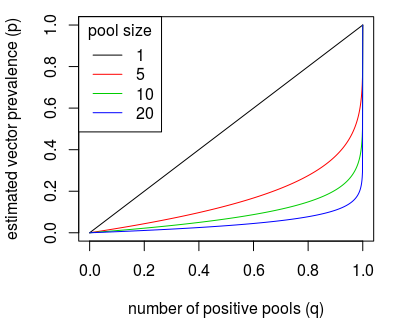
\includegraphics[height=6cm]{Figures/IndVsPool}
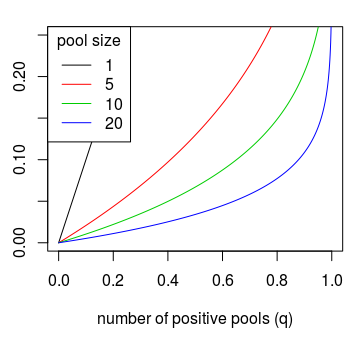
\includegraphics[height=6cm]{Figures/IndVsPoolZoom}
\end{array}$
\end{center}
\caption[Pool prevalence vs. actual prevalence.]{The relationship between vector prevalence ($p$) and pool prevalence ($q$) for different pool sizes if we assume large number of pools ($M$). Top: The relationship for all pool and vector prevalences. Bottom: Zoomed in on 0 - 20\% vector prevalence.}
\label{fig:pool}
\end{figure}

Figure \ref{fig:xeno} shows the reviewed data from Egypt \cite{Farid2007,Ramzy2006}, PNG \cite{Reimer2013_insecticidal,Weil2008} and Ghana \cite{Owusu2015} on a graph showing the relationship between vector prevalence and human mf prevalence for different proportions of parous mosquito (45\%, 60\% and 75\%). These studies all estimated vector prevalence from pooled prevalences, using similar methods to what we have described here, via commonly-used software tool PoolScreen. The lower part of the figure focuses on regions of low prevalence ($<10$\%), for which the model relationship is close to linear. Linear regression fits to the data show the differences between settings, indicating systematic differences in the mosquito dynamics. Even within one country, for example looking at Giza (yellow) and Qalubiya (red) there are potentially significant differences in the proportion of vectors that are parous. This reiterates the importance of having robust and well-characterised methods, involving understanding of the underlying dynamics, when interpreting vector measures of disease for public health applications.

\begin{figure}[ht]
\begin{center}$
\begin{array}{cc}
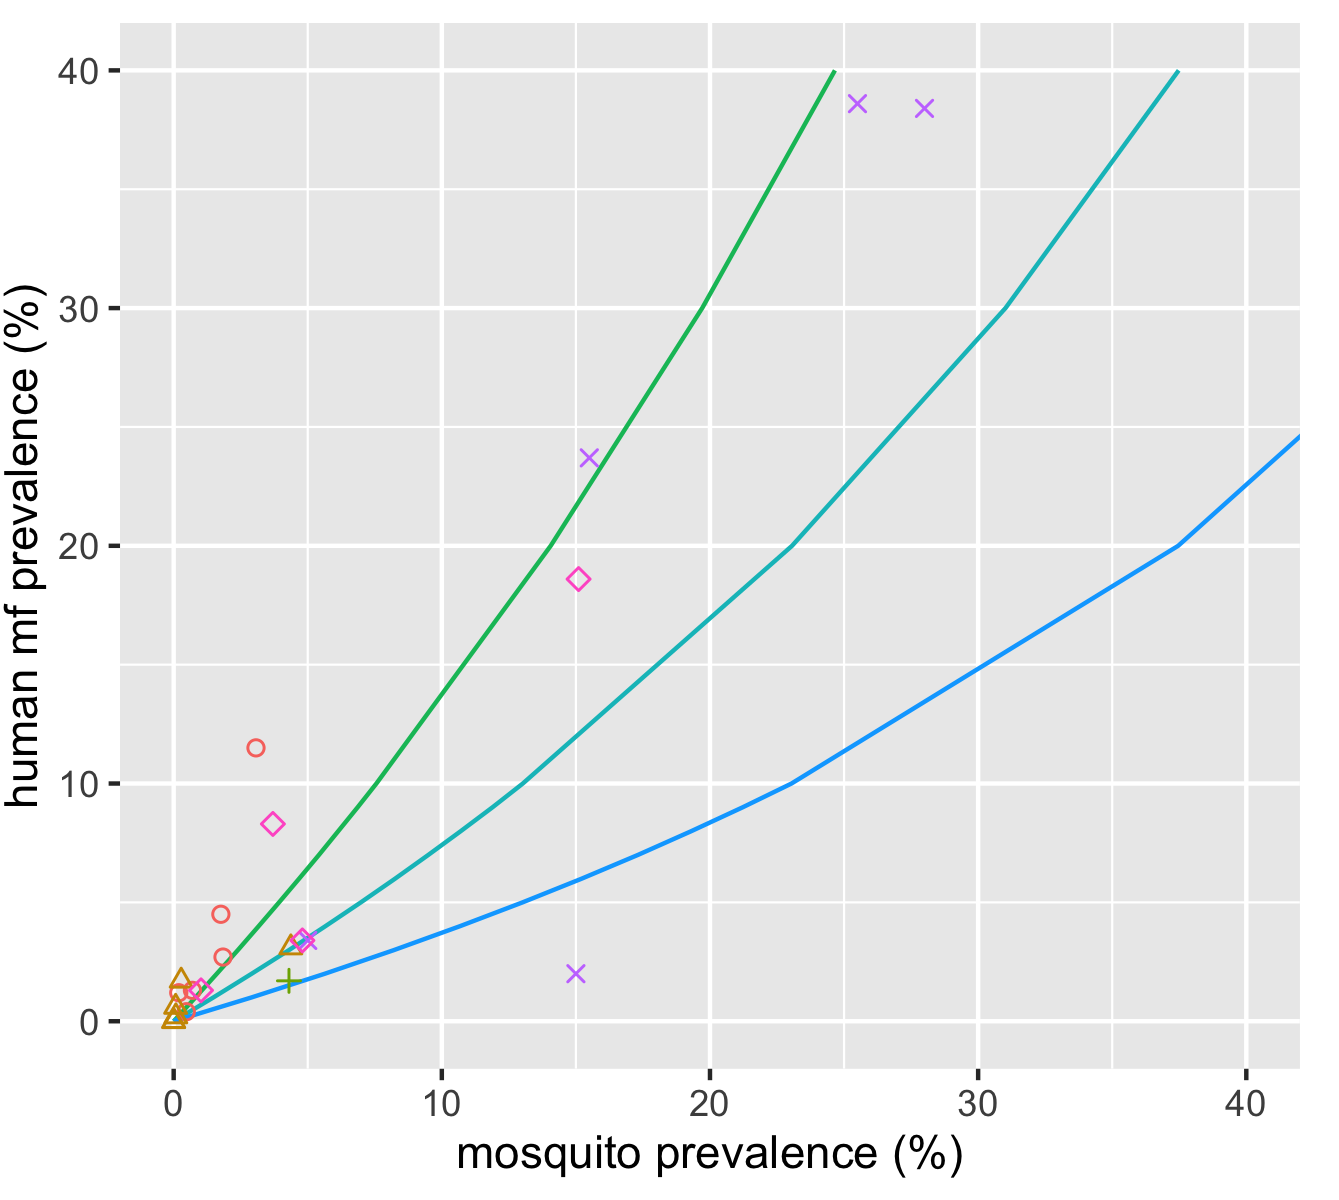
\includegraphics[height=6cm]{Project/Figures/Xeno/mfPrev_crop.png}
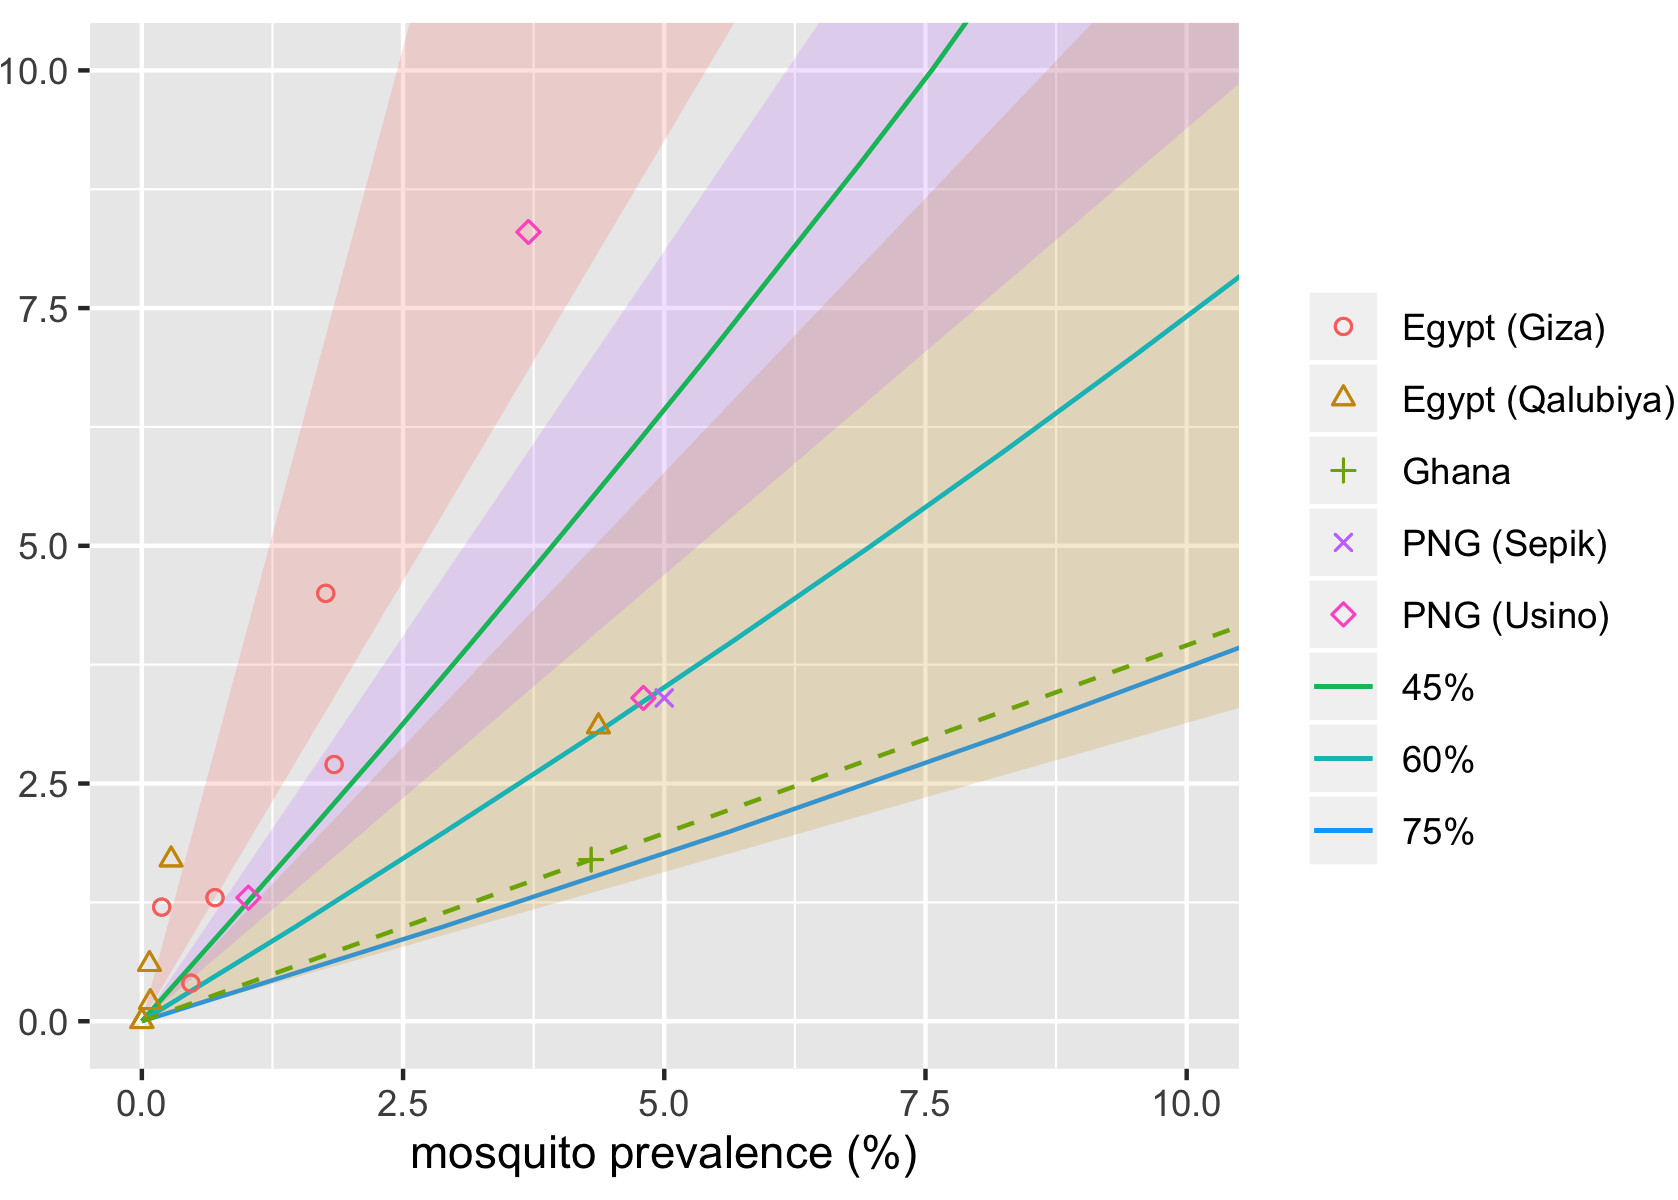
\includegraphics[height=6cm]{Project/Figures/Xeno/mfPrevZoomFit_crop.png}
\end{array}$
\end{center}
\caption[Xenomonitoring data with model comparison.]{Data and model linking vector prevalence and individual prevalence for different parity levels. In the data vector prevalence is estimated from pooled prevalence and the model shows curves for a range of parity (45\%, 60\% and 75\%). Right: Zoomed in to low prevalence ($<10$\%) with shaded regions representing uncertainty of fitted linear regressions to: a) Giza, Egypt \cite{Farid2007,Ramzy2006} (Red), b) Qalubiya, Egypt \cite{Farid2007,Ramzy2006} (yellow), c) Sepik \cite{Reimer2013_insecticidal} and Usino \cite{Weil2008}, PNG (purple). A dashed line shows the best fit for Ghana \cite{Owusu2015} but uncertainty cannot be calculated due to sample size.}
\label{fig:xeno}
\end{figure}

\begin{figure}[ht]
\begin{center}
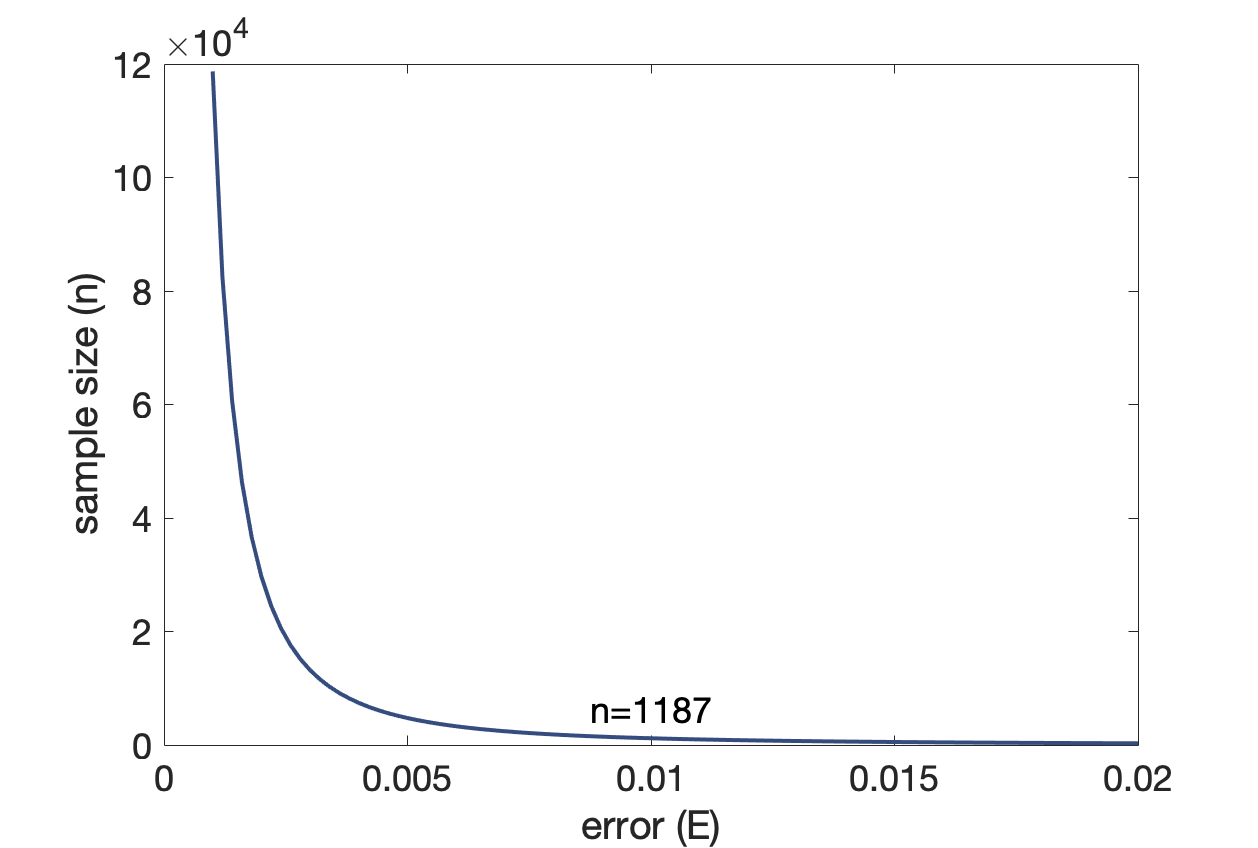
\includegraphics[height=7cm]{Project/Figures/Xeno/VaryError.png}
\end{center}
\caption[Sample size calculations.]{Plot showing how required sample size, $n$, of parous vectors varies with chosen error, $E$. Required sample size of random vectors, e.g. using light traps, is $m=an$. Here we take $a=10$ and the total number of vectors that need to be sampled is given by $n + m = n+an$.}
\label{fig:error}
\end{figure}

We are interested in the use of vector prevalence (either pooled or individual) ratios across trap types to estimate host prevalence, in particular whether required sample sizes are feasible for use of xenomonitoring as a surveillance method. Figure \ref{fig:error} shows how the required parous vector (gravid trap) sample size, $n$, varies with the size of the allowable error margin, $E$. A 1\% host mf prevalence error margin gives a required sample size of 1187 parous vectors, which translates to 11870 additional random vectors, giving an overall sample size of 13057 vectors. A smaller margin gives larger sample sizes; an error of 0.1\% prevalence giving sample sizes of $n=118,700$, $m=1,187,000$ and an overall sample size of 1,305,700.

\FloatBarrier

Using the relationships derived in this chapter we can run trial sampling scenarios, with fixed sample size and host prevalence, to compare the different methods of characterising uncertainty. A series of trial sampling scenarios were run with host prevalence $H=0.01$ or 1\% mf prevalence, a sample size of $n=1187$ and $m=11870$, as recommended by our sample size calculations, and a range of parity between 0.1 and 0.75. 

Figure \ref{fig:parity} shows parity estimates plotted against true underlying parity, with confidence intervals calculated using the Ln method (orange) and Delta method (blue). The main difference between the methods is that the Ln method is non-symmetrical around the central estimate, which in most cases leads to a narrower lower interval and a wider upper interval. However, aside from this small shift, there is generally good agreement between the two methods. The Delta method is the most widely used in statistics and is generalisable to more complex functions of random variables, so this method is the one that we use going forward.

\begin{figure}[ht]
\begin{center}
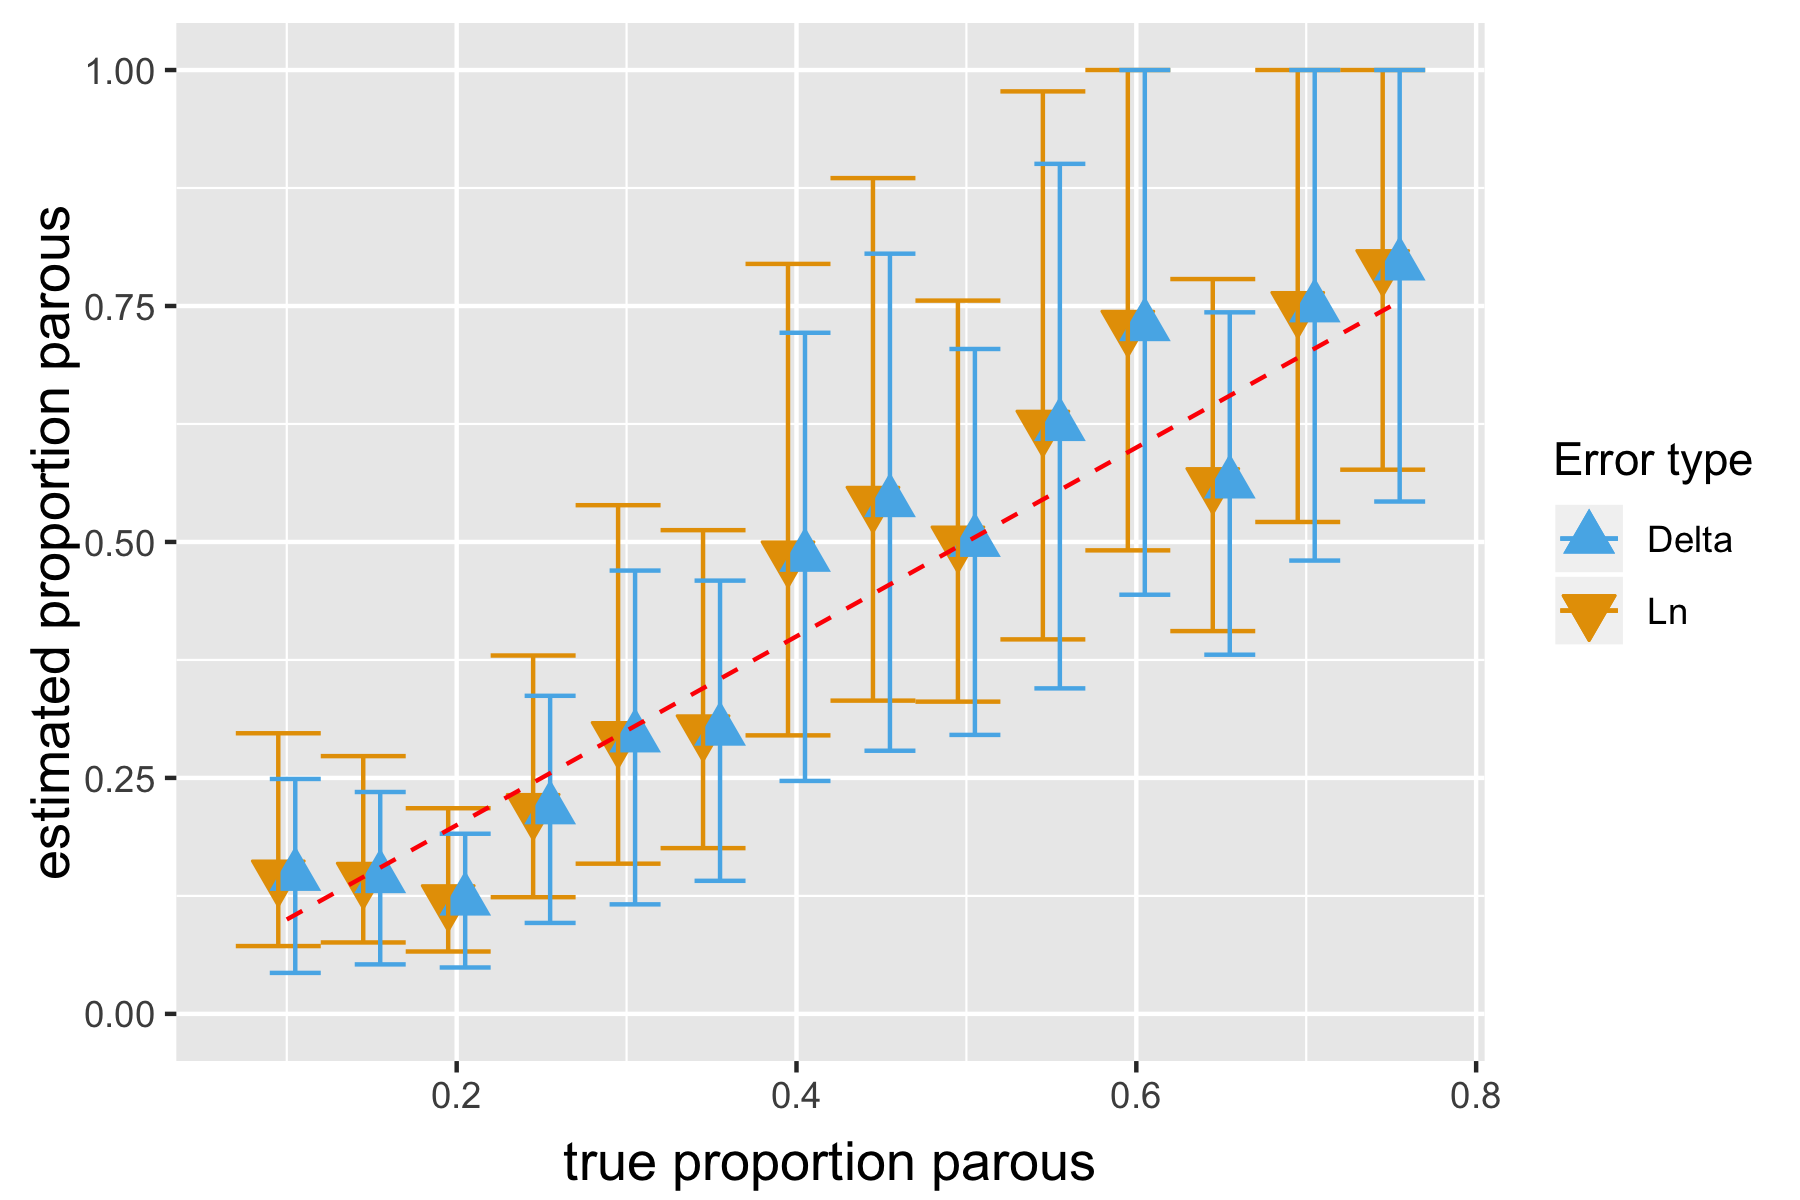
\includegraphics[height=8cm]{Project/Figures/Xeno/ParousEst.png}
\end{center}
\caption[Estimated vs. true proportion parous.]{Example simulation showing comparison between the two methods of confidence interval derivation for proportion of population parous when calculated from observed vector prevalence in gravid and random traps: Ln (orange, triangle) and Delta (blue, inverted triangle). Sample sizes: $n=1187$, $m=11870$ and underlying host prevalence $H=0.01$. Data points are offset to allow ease of viewing, neighboring points represent the same parous proportion.}
\label{fig:parity}
\end{figure}

Figure \ref{fig:vPrev} shows the estimated vector prevalence plotted against true vector prevalence for parous (orange) and random (blue) sampling of the population, with confidence intervals calculated using the Delta method. The randomly sampled vectors will include nulliparous mosquitoes which cannot test positive for LF presence as they haven't yet taken a bloodmeal, hence the random prevalence will always be less than the parous prevalence. As the sampling method takes into account trap efficiency, we have sampled ten times the number of random vectors as parous vectors, meaning the confidence intervals on these are narrower. However, the parous prevalence estimates are all within 0.5\% prevalence of the true value and the sampled data matches the true underlying value well.

\begin{figure}[ht]
\begin{center}
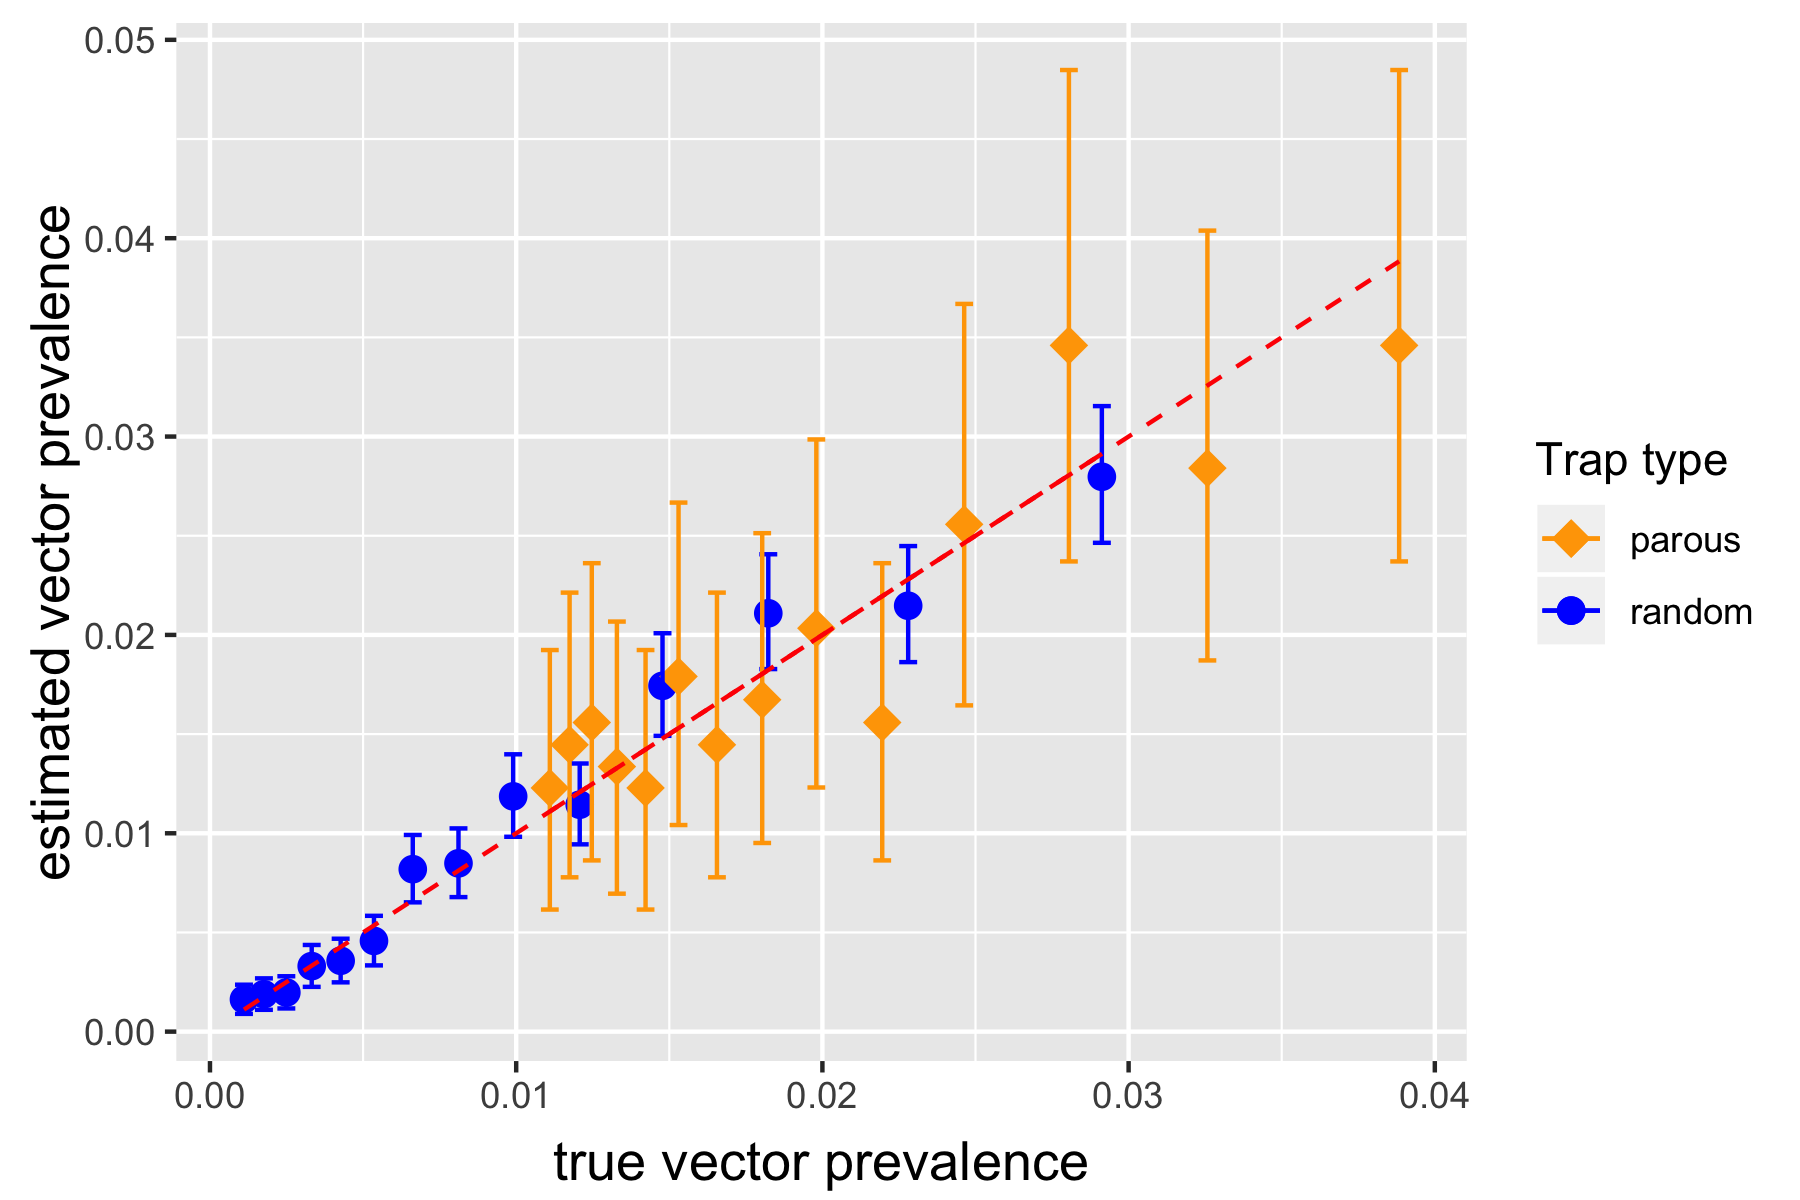
\includegraphics[height=8cm]{Project/Figures/Xeno/VPrevEst.png}
\end{center}
\caption[Estimated vector prevalence (parous and random).]{Example simulation showing the estimated vector prevalence in parous (orange, diamond) and random (blue, circle) populations, with sample sizes $n=1187$ and $m=11870$ respectively and underlying host prevalence $H=0.01$. Confidence intervals were calculated using the Delta method.}
\label{fig:vPrev}
\end{figure}

The next step is to consider the confidence intervals around the estimated host prevalence (see Figure \ref{fig:hPrev}). We compare the results of sampling individual vectors (red) and pooling the same number of total vectors into pools of $N=20$ (blue). This gives different estimates of host prevalence for the same underlying prevalence (1\%) and parity, and the Delta method was again used to calculate confidence intervals. In all cases, as expected due to loss of information through pooling, the pooled confidence intervals are either equivalent or wider than the individually sampled intervals. However, there is actually surprisingly little deviation in both the central estimates and confidence intervals between the two methods. This is potentially due to the simple near-linear relationship between pool prevalence and vector prevalence at low prevalence levels (Figure \ref{fig:pool}). Pooling vectors for testing is substantially cheaper and less labour intensive, so this could be exploited to increase feasibility of xenomonitoring as a survey tool.

The majority of the confidence intervals from individually tested vectors are less than 1\% prevalence on either side of the estimated host prevalence, whereas some of the confidence intervals from pooled testing are closer to 1.5\% each side. If pooling was being used then a larger sample size would be required for the same error width, but this would likely still represent fewer overall lab tests than using this sample size and individual testing.

\begin{figure}[ht]
\begin{center}
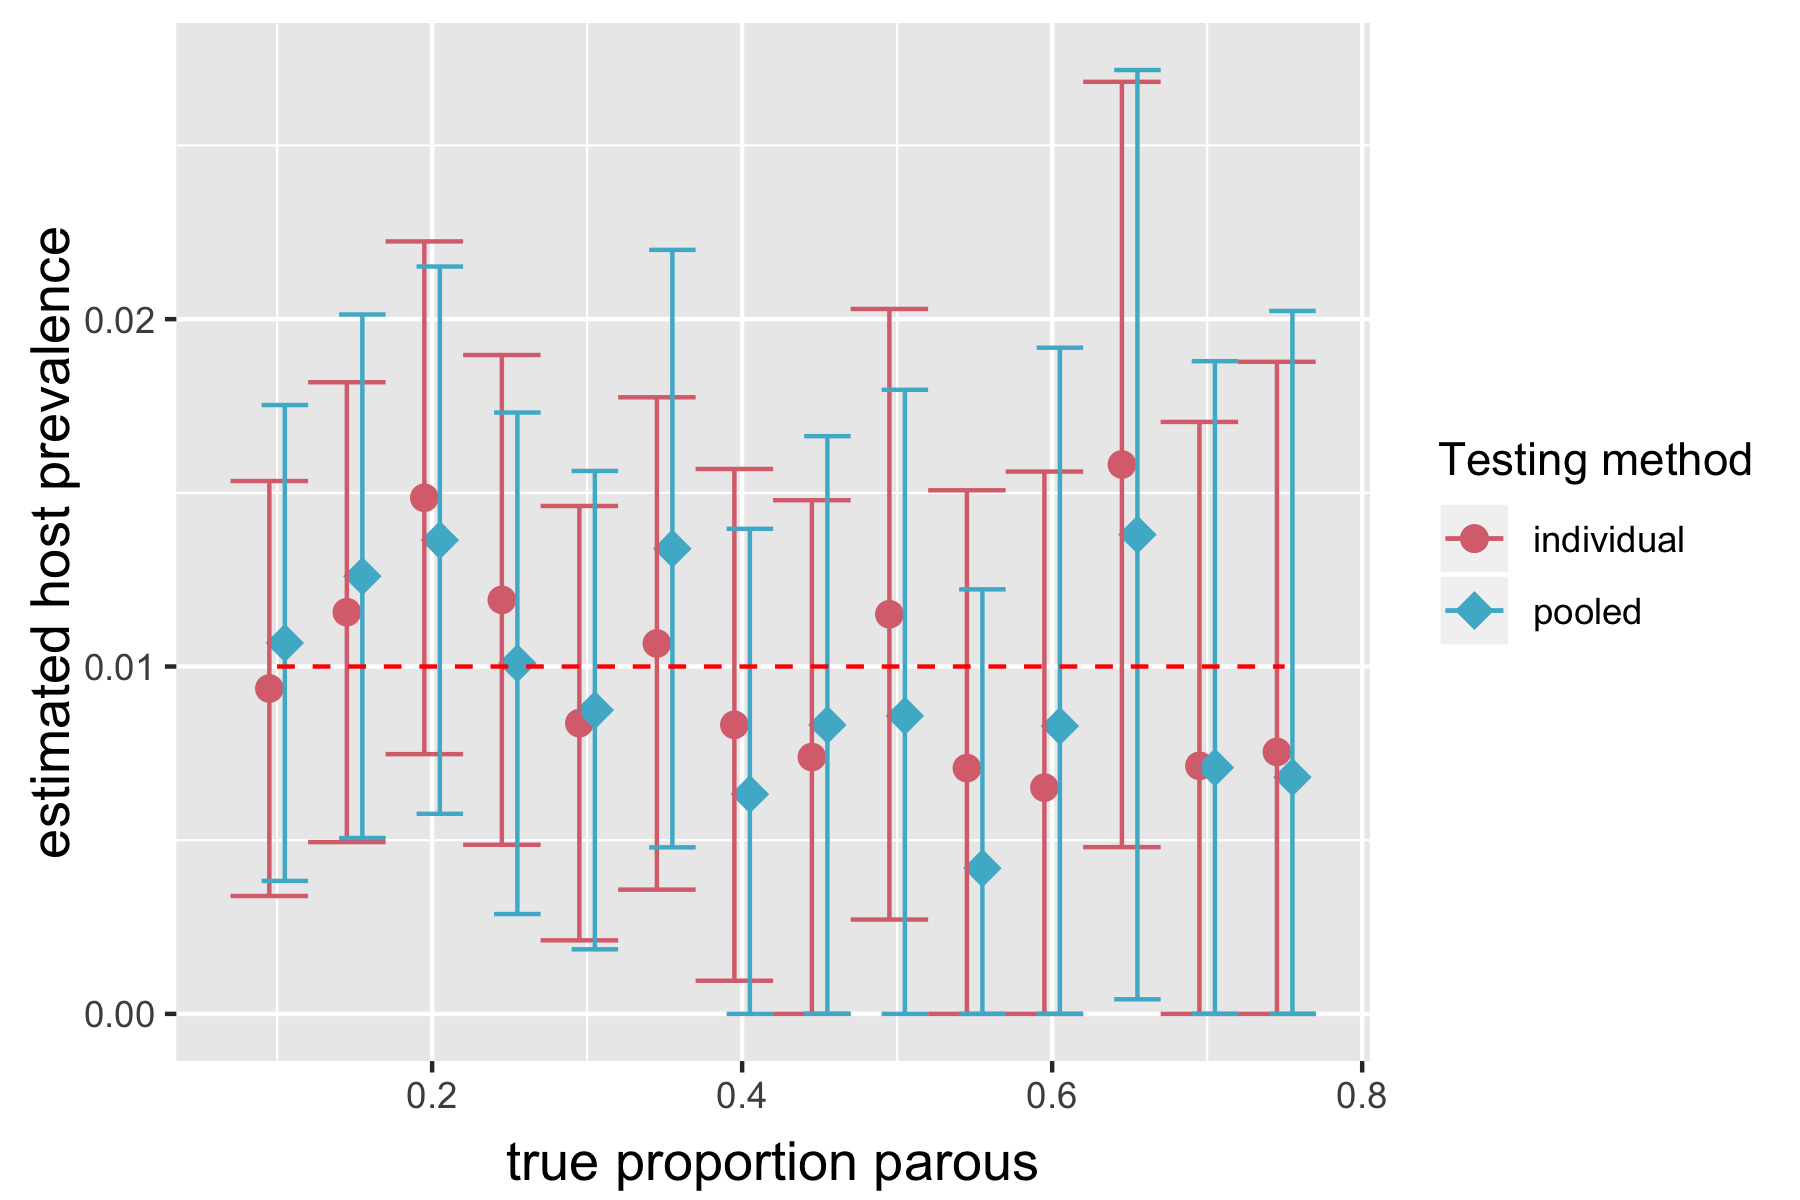
\includegraphics[height=9cm]{Project/Figures/Xeno/HPrevEst.png}
\end{center}
\caption[Estimated host prevalence (individual and pooled testing).]{Example simulation showing comparison of estimated host prevalence for individual (red, circle) and pooled (blue, diamond) tested mosquitoes. Sample sizes $n=1187$ and $m=11870$ respectively in both cases, with a pool size of $N=20$ in the pooled case, and underlying host prevalence $H=0.01$. Confidence intervals were calculated using the Delta method. Data points are offset to allow ease of viewing.}
\label{fig:hPrev}
\end{figure}

\FloatBarrier

\section{Discussion}

Through deriving analytical expressions for host prevalence as a function of vector DNA prevalence and subsequent confidence intervals, we have been able to calculate the vector sample sizes required to measure host prevalence to within a specified error with 95\% confidence. We have also demonstrated the potential of exploiting biases in different commonly used CDC-approved trap types as a proxy for measuring the proportions of nulliparous and parous mosquitoes, an essential locally-dependent parameter of vector and transmission dynamics. We also generalised these results to include the potential for pooling vectors before carrying out laboratory testing, which could substantially reduce costs and increase feasibility. These results are also directly applicable to other mosquito-borne diseases, such as malaria, as the biological details of LF are not used anywhere in this analysis.

We found that the relationship between pool prevalence and vector prevalence would be hard to use for mid to high vector prevalences ($>$20\% prevalence) due to the rapidly increasing slope. This would mean a small change in observed pool prevalence would lead to an increasingly large change in estimated vector prevalence, making it difficult to calculate vector prevalence to within a sensible error. However, at low vector prevalence ($<$20\%) this calculation becomes much more feasible, even for pool sizes of up to 20 vectors, and at very low prevalence ($<$5\%) the relationship between pool prevalence and vector prevalence is close to linear, allowing for very easy calculation.

Comparing the model of host prevalence as a function of prevalence to data observed in field studies demonstrated that parous proportions may vary significantly between settings, potentially due to local differences in the environment or vector dynamics.

When considering the required sample sizes used to measure vector and parous vector prevalence we estimated that a total sample size of just over 13,000 vectors (1187 parous, 11870 random) would be required to measure host prevalence to within an error of 1\% mf prevalence. This is a relatively large, but not infeasible, sample size. However, the required sample size increases exponentially with decreasing error, meaning the required precision of surveillance will be a key determining factor in whether xenomonitoring is a feasible method for post-MDA settings.

Cost of surveillance is also a key factor when programs consider which method to use. Both collection and PCR testing of mosquitoes are currently relatively high in cost due to the necessity of expensive real-time PCR machines \cite{Goodman2003} and skilled labour \cite{Okorie2016}, meaning individual capture and testing of vectors is likely to be infeasible in most settings. However, human surveillance is also a high cost intervention and is mainly used in post-MDA scenarios, where the low prevalences mean sample sizes need to be both large and spatially-distributed to effectively estimate presence or absence of transmission \cite{WHO2011}. The development of rapid point-of-care tests such as the filarial test strip (FTS) has alleviated some of these challenges, but many programs find there is a lack of willingness in the population to participate in surveillance for an infection is no longer considered a major problem \cite{Pilotte2016}.

Pooling vectors is common practice in the field, particularly if resources are limited, and can save substantially on PCR costs \cite{Okorie2016}. Our first investigations suggest that the difference in confidence between individually testing and pooling vectors is relatively small, potentially due to the low prevalence settings considered. We would expect this difference to be increased for higher prevalences, but as the main interest in xenomonitoring comes from elimination settings, pool sizes of up to 20 vectors in these places should only lead to a small loss of accuracy. More work needs to be done to directly link required sample size, pool size and error width. 

It is important to note that our assumption of zero co-variance between trap type samples only holds if traps are not set at the same time in the same place, as we might expect the presence of multiple trap types in one location to bias the samples. We have also assumed that the same number of vectors are included in each pool, which is not always the case in vector studies, often the average pool size is quoted instead. Further investigation would need to be done as to how feasible it is to fix pool size in the field and how variation in pool size might impact our calculations.

As more countries achieve EPHP and move into post-MDA surveillance, novel tools for monitoring infection levels become increasingly important. Human-based testing is expensive and invasive, with high associated labour and resource costs, and xenomonitoring has long been discussed as a potentially financially viable alternative but there is still little understanding of the relationship between vector prevalence and host prevalence and common opinion is that sample sizes may be logistically infeasible. We have attempted to bridge this knowledge gap and our findings suggest that sample sizes may be more feasible than expected, depending on required precision levels. However, we have presented analysis of one potential xenomonitoring surveillance method, further modelling and field work will be needed to investigate and compare a range of methods in developing the best tools for surveillance in the journey towards true elimination of transmission.

\subsection{Chapter Summary}

In this chapter I derived analytical relationships between host prevalence and measurable parasite DNA prevalence in vector blood meals, considering both individually sampled and pooled vector measurements. I also described a method for estimating the proportion of parous mosquitoes. I also derived an explicit formula for sample size calculation, depending on a required precision. My results show that required sample sizes may be more feasible than previously expected, and that pooling vectors may be a viable method for reducing the costs and labour required for use of xenomonitoring as a surveillance tool.

\FloatBarrier